%--------------------------------------------------------------------------------
% Constrói a capa com base na seção de identificação do main.tex
%--------------------------------------------------------------------------------
\begin{capa}
\center
	
\includegraphics[scale=0.6]{img/univasf.jpg}

	{\ABNTEXchapterfont\bfseries\large\imprimirinstituicao}

	\vspace*{5cm}
	{\ABNTEXchapterfont\bfseries\large\imprimirautor}

	\vfill
	{\ABNTEXchapterfont\bfseries\large\imprimirtitulo}
	\vfill
	\ABNTEXchapterfont\bfseries\large\imprimirlocal\\ \the\year

	\vspace*{1cm}

\end{capa}
%--------------------------------------------------------------------------------
% Constrói a folha de rosto com base na seção de identificação do main.tex
%--------------------------------------------------------------------------------
\begin{folhaderosto}
\center
		{\ABNTEXchapterfont\bfseries\large\imprimirautor}
		\vspace*{\fill}

		{\ABNTEXchapterfont\bfseries\large\imprimirtitulo}
		\vspace*{\fill}

		{\hspace{.45\textwidth}
		\begin{minipage}{.5\textwidth}
			\SingleSpacing
			\imprimirpreambulo \\ \\

			{\imprimirorientadorRotulo~\imprimirorientador\par}
			{\imprimircoorientadorRotulo~\imprimircoorientador\par}

		\end{minipage}%
		\vspace*{\fill}}%
		\vspace*{\fill}
			\ABNTEXchapterfont\bfseries\large\imprimirlocal\\ \the\year
		\vspace*{1cm}
\end{folhaderosto}

%--------------------------------------------------------------------------------
% Constrói a ficha catalográfia com base na seção de identificação do main.tex
% Está comentado porque no final das contas a biblioteca do seu campus que gera a 
% numeração, você pode adicionar os numeros aqui, ou anexar o pdf gerado por eles
% ao documento.
%--------------------------------------------------------------------------------
%\begin{fichacatalografica}
%	\vspace*{\fill}					% Posição vertical
%	\hrule							% Linha horizontal
%	\begin{center}					% Minipage Centralizado
%	\begin{minipage}[c]{12.5cm}		% Largura
%
%	\imprimirautor
%
%	\hspace{0.5cm} \imprimirtitulo  / \imprimirautor. --
%	\imprimirlocal, \the\year-
%
%	\hspace{0.5cm} xx p. : il. (algumas color.) ; 30 cm.\\
%
%	\hspace{0.5cm} \imprimirorientadorRotulo~\imprimirorientador\\
%
%	\hspace{0.5cm}
%	\parbox[t]{\textwidth}{\imprimirtipotrabalho~--~\imprimirinstituicao,
%	\the\year.}\\
%
%	\hspace{0.5cm}
%		1. Palavra-chave1.
%		2. Palavra-chave2.
%		I. Orientador.
%		II. Universidade xxx.
%		III. Faculdade de xxx.
%		IV. Título\\
%
%	\hspace{8.75cm} CDU 02:141:005.7\\
%
%	\end{minipage}
%	\end{center}
%	\hrule
%\end{fichacatalografica}

%--------------------------------------------------------------------------------
% Anexando a ficha catalogáfica e a folha de aprovação 
%--------------------------------------------------------------------------------
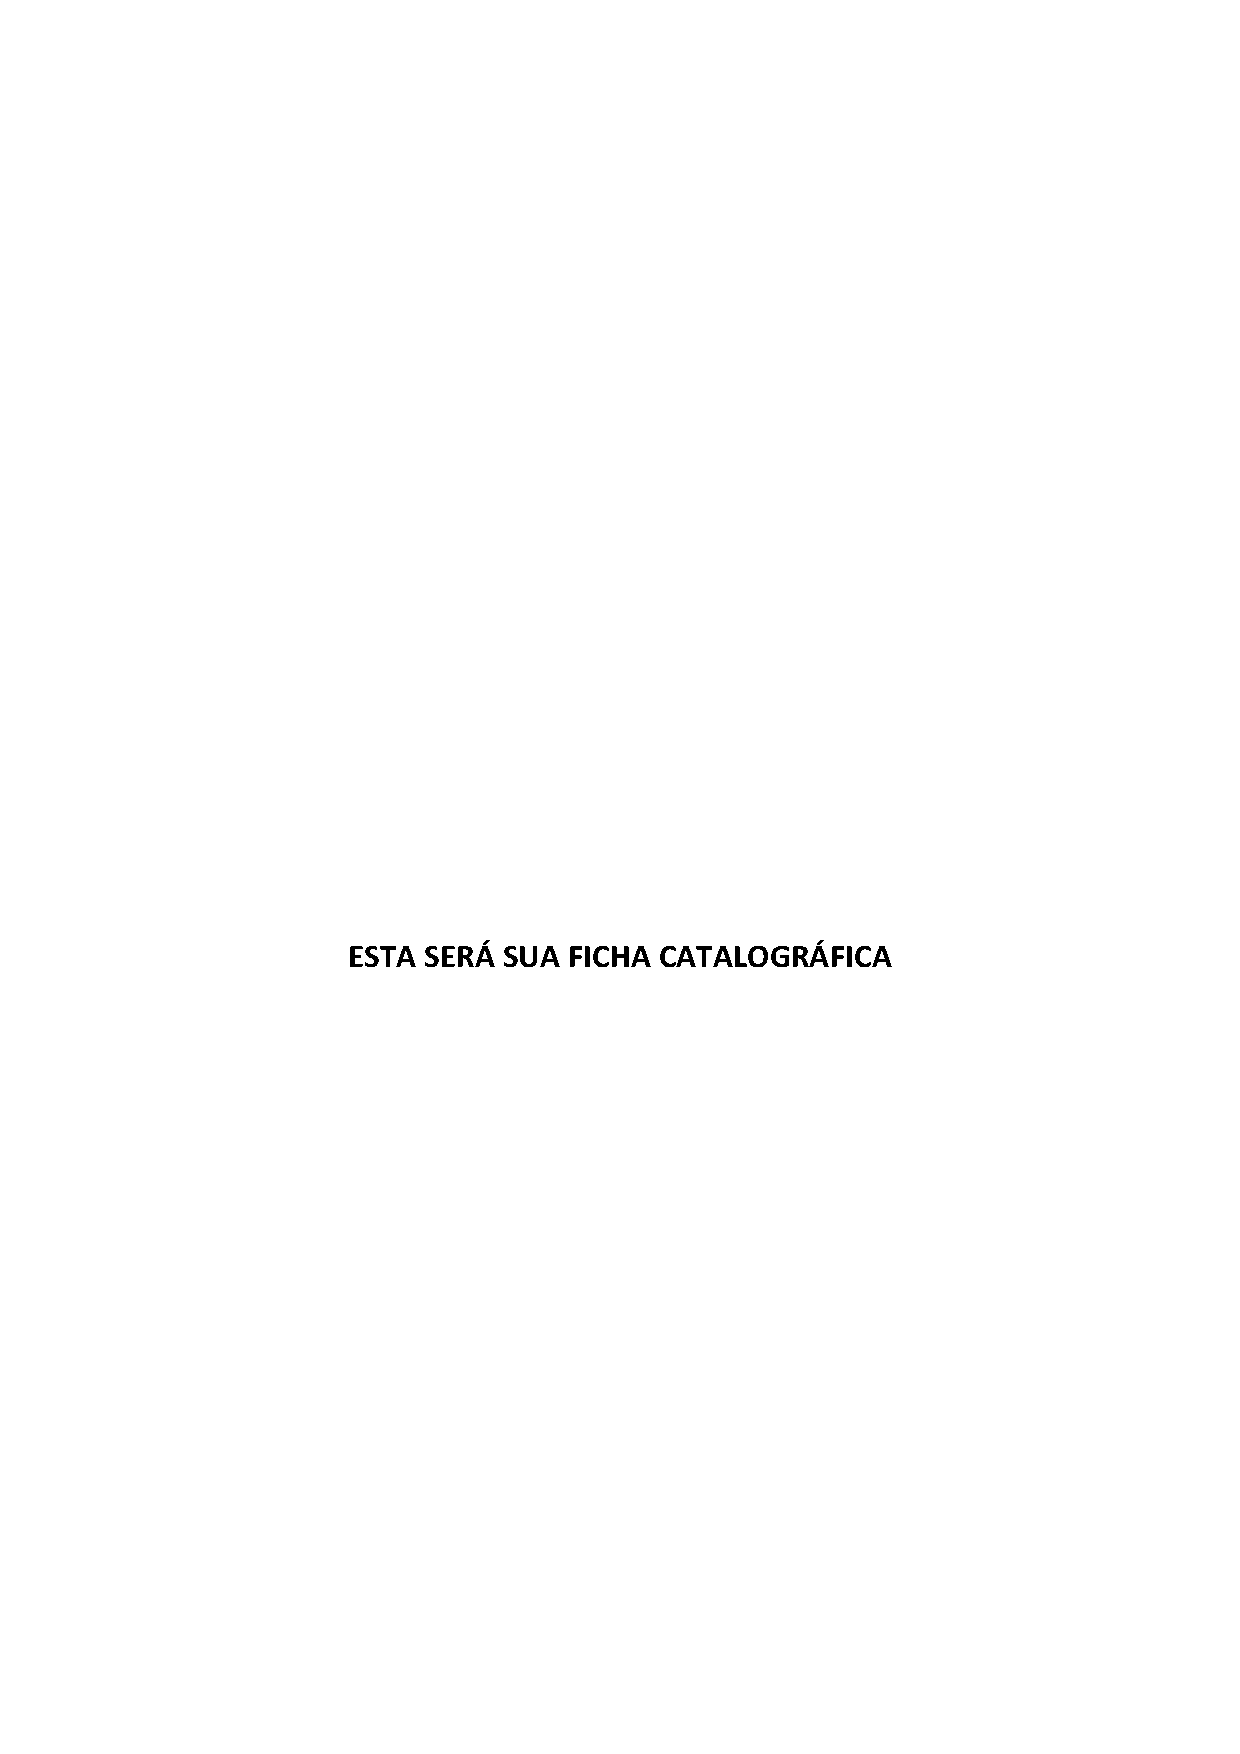
\includepdf[pages=-]{anexos/ficha.pdf}

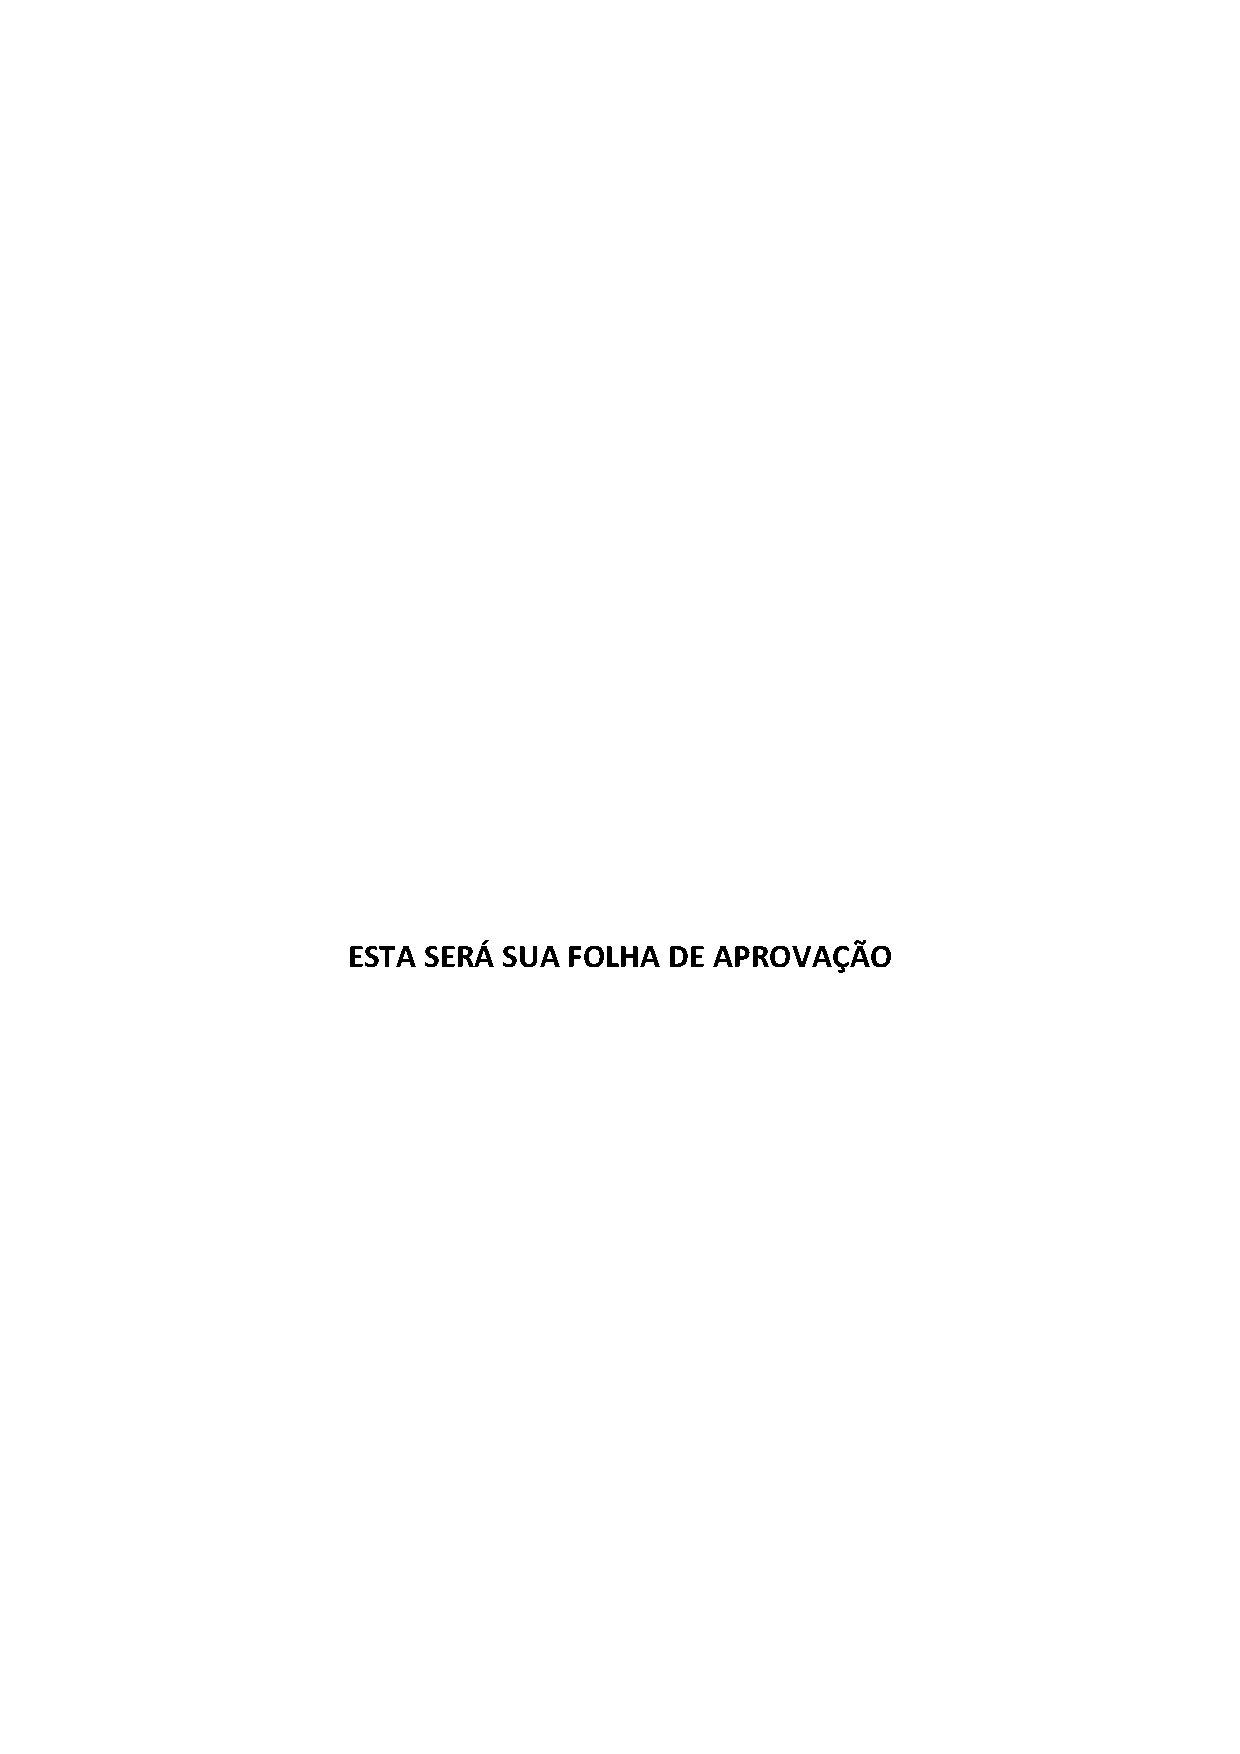
\includepdf[pages=-]{anexos/aprovacao.pdf}

\setlength{\ABNTEXsignwidth}{12cm}

%--------------------------------------------------------------------------------
% Está comentado pelo mesmo motivo da ficha catalográfica 
%--------------------------------------------------------------------------------
%\begin{folhadeaprovacao}
%	\begin{center}
%	    {\ABNTEXchapterfont\bfseries\large\imprimirinstituicao}
%	    \vspace*{\fill}
%
%	    {\ABNTEXchapterfont\bfseries\large FOLHA DE APROVAÇÃO}
%	    \vspace*{\fill}
%
%	    {\ABNTEXchapterfont\bfseries\large\imprimirautor}
%
%	    \vspace*{\fill}\vspace*{\fill}
%	    {\ABNTEXchapterfont\bfseries\large\imprimirtitulo}
%	    \vspace*{\fill}
%
%	    {\hspace{.45\textwidth}
%		\begin{minipage}{.5\textwidth}
%			\SingleSpacing
%			\ABNTEXchapterfont\imprimirpreambulo \\ \\
%
%			{\ABNTEXchapterfont\imprimirorientadorRotulo~\imprimirorientador\par}
%			{\ABNTEXchapterfont\imprimircoorientadorRotulo~\imprimircoorientador\par}
%
%		\end{minipage}%
%	    \vspace*{\fill}}
%	\end{center}
%
%	\vspace*{\fill}	
%	
%	\begin{center}
%			 \ABNTEXchapterfont\large Aprovado em: \_\_\_\_ de \_\_\_\_ de 2017
%	\end{center}

%	\vspace*{\fill}
	
%	\begin{center}
%			 \ABNTEXchapterfont\bfseries\large Banca Examinadora
%	\end{center}
%		
%   \ABNTEXchapterfont\assinatura{Fábio Nelson de Sousa Pereira, Mestre, Universidade Federal do Vale do São Francisco}
%	\ABNTEXchapterfont\assinatura{Jorge Luis Cavalcanti Ramos, Doutor, Universidade Federal do vale do São Francisco}
%  \ABNTEXchapterfont\assinatura{Ricardo Argenton Ramos, Doutor, Universidade Federal do Vale do São Francisco}
%	 \vspace*{\fill}

	 
%\end{folhadeaprovacao}

%--------------------------------------------------------------------------------
% Insere a epígrafe
%--------------------------------------------------------------------------------
% \newpage
% \vspace*{\fill}
% \begin{flushright}
% 		\textit{Lorem Ipsum...}
% \end{flushright}

%--------------------------------------------------------------------------------
% Seção de agradecimentos
%--------------------------------------------------------------------------------
% \begin{agradecimentos}
	
% \lipsum[2-4]

% \end{agradecimentos}

%--------------------------------------------------------------------------------
% Insere a segunda epígrafe
%--------------------------------------------------------------------------------
% \begin{epigrafe}
%     \vspace*{\fill}
% 	\begin{flushright}
% 		Se pude enxergar a tão grande distância, foi subindo nos ombros de gigantes.\\
% 		 \vspace{\baselineskip}
% 		\textbf{Isaac Newton}\\
% 		\textbf{Carta à Robert Hooke, 1676}
% 	\end{flushright}
% \end{epigrafe}



%--------------------------------------------------------------------------------
% Seção de resumos
%--------------------------------------------------------------------------------
% resumo em português
\setlength{\absparsep}{18pt} % ajusta o espaçamento dos parágrafos do resumo
\begin{resumo}

Um dos atributos mais significativos para a garantia da qualidade de uma fruta é a quantidade de açúcares nela contida. Entretanto, para a obtenção deste valor, é 
exigida a destruição da amostra, de forma que seu conteúdo seja analisado. Essa abordagem, além de destrutiva, é onerosa; assim, o emprego de um sistema de visão 
computacional para previsão desta variável de saída mostra-se vantajoso. Entretanto, é necessário definir as variáveis visuais da fruta a partir das quais o teor 
de sólidos solúveis será obtido. Assim, foi conduzido um estudo baseado em diferentes artigos onde é empregado o processamento de imagens para predição de atributos
 de qualidade. A fruta analisada foi a manga, da variedade ‘Palmer’, por ser produzida em abundância no Vale do São Francisco e por contribuir para a economia de 
 Juazeiro (BA) e Petrolina (PE) através de sua exportação. As melhores técnicas de pré-processamento e inferência também foram avaliadas, de forma a obter a melhor 
 abordagem para predição de sólidos solúveis em manga. Foi encontrado que as melhores técnicas de pré-processamento foram filtro da mediana, operações de abertura e fechamento e limiarização simples. Os atributos visuais mais significantes foram a dimensão de correlação, taxa R/B e as médias do canal B na região equatorial e da haste. O coeficiente de correlação foi igual a 0,9752, obtido através da \textit{Random Forest}.

 \textbf{Palavras-chave}: Quantidade de açúcares. Visão computacional. \textit{Random Forest}.

\end{resumo}

%---------------------------------------------------------------------------------
% resumo em inglês
\begin{resumo}[Abstract]
\begin{otherlanguage*}{english}

One of the most significant attributes for guaranteeing the quality of a fruit is the amount of sugars contained in it. However, to obtain this value, the destruction 
of the sample is required, so that its content is analyzed. This approach, besides being destructive, is onerous; thus, the use of a computer vision system to predict 
this output variable is advantageous. However, it’s necessary to define the fruit’s visual variables from which the sugar content will be obtained. Thus, the study 
was conducted based on different articles in which image processing is employed to predict quality attributes. The analyzed fruit was the mango, from ‘Palmer’
 variety, due to its abundant production in the São Francisco Valley and its contribution to the economy in Juazeiro (BA) and Petrolina (PE) through exportation. 
 The best pre-processing and inference techniques were also evaluated in order to obtain the best approach to predict sugars in mangoes. It was found that the best pre-processing techniques were median filter, opening and closing operations and thresholding. The most significant visual aspects were the correlation dimension, R/B rate and the B channel mean in the stalk and apex regions. The correlation coefficient was equal to 0,9752 and was obtained through Random Forest.

	\vspace{\onelineskip}

	\noindent
	\textbf{Key-words}: \textit{Sugar content. Computer vision. Random Forest}.

\end{otherlanguage*}
\end{resumo}


%---------------------------------------------------------------------------------
% Insere lista de ilustrações
%---------------------------------------------------------------------------------
\begin{KeepFromToc} % Este comando evita que todas as seções dentro dele de apareçam no sumário
\pdfbookmark[0]{\listfigurename}{lof}
\listoffigures
%\addcontentsline{toc}{chapter}{Lista de Figuras}
\cleardoublepage


%---------------------------------------------------------------------------------
% Insere lista de tabelas
%---------------------------------------------------------------------------------
\pdfbookmark[0]{\listtablename}{lot}
\listoftables
\cleardoublepage

%---------------------------------------------------------------------------------
% Ajusta lista de código - alterar de figures para códigos - by @Gabrielr2508
%---------------------------------------------------------------------------------
% \makeatletter
% \let\l@listing\l@figure
% \def\newfloat@listoflisting@hook{\let\figurename\listingname}
% \makeatother

%---------------------------------------------------------------------------------
% Insere lista de códigos - by @leolleocomp
%---------------------------------------------------------------------------------
% \listoflistings

\end{KeepFromToc}

%---------------------------------------------------------------------------------
% Insere lista de abreviaturas e siglas
%---------------------------------------------------------------------------------
\begin{siglas}
	\item[BCD]		Dimensão de contagem de caixa – \textit{Box Counting Dimension}
	\item[CCD]		Dispositivo de carga acoplada – \textit{Charge-coupled Device}
	\item[CD]		Dimensão de correlação – \textit{Correlation Dimension}
	\item[DD]		Dimensão de dilatação – \textit{Dilation Dimension}
	\item[LS-SVM]		Máquina de vetores de suporte por mínimos quadrados – \textit{Least-Squares Support Vector Machine}
	\item[MDA]		Análise discriminante múltipla – \textit{Multiple Discriminant Analysis}
	\item[MLR]		Regressão linear múltipla – \textit{Multiple Linear Regression}
	\item[PCA]		Análise de componentes principais – \textit{Principal Component Analysis}
	\item[RBF]		Função de base radial – \textit{Radial Basis Function}
	\item[RMSE]		Raiz do erro quadrático médio – \textit{Root Mean Square Error}
	\item[RFE]		Eliminação recursiva de atributos - \textit{Recursive Feature Elimination}
	\item[RNA]		Rede neural artificial
	\item[RPI]		\textit{Ripening Index}
	\item[RSS]		Soma do quadrado dos resíduos – \textit{Residual Sum of Squares}
	\item[SST]		Sólidos solúveis totais
	\item[SVM]		Máquina de vetores de suporte – \textit{Support Vector Machine}
	    
\end{siglas}

%---------------------------------------------------------------------------------
% Insere o sumario
%---------------------------------------------------------------------------------
\pdfbookmark[0]{\contentsname}{toc} 
\tableofcontents*
\cleardoublepage
